\documentclass[11pt]{book}

\usepackage[book, es]{../cuevasthm}
\input{../template.tex}
% \input{../code.tex}

\usepackage{minted}
\usemintedstyle{colorful}
\setminted{
	mathescape,
	linenos,
	autogobble,
	bgcolor=black!5,
	fontsize=\small
}

\usepackage{subfiles}

% Bibliografía
% \DeclareBibliographyCategory{elementary}
% \addtocategory{elementary}{khinchin:fractions, niven:irrational, hua:number, mordell:diophantine}
% \defbibheading{elementary}{\section*{Teoría elemental de números}}

% \DeclareBibliographyCategory{analytic}
% \addtocategory{analytic}{chan:analytic, bateman:analytic, overholt:analytic, tenenbaum:analytic}
% \defbibheading{analytic}{\section*{Teoría analítica de números}}

% \DeclareBibliographyCategory{algebraic}
% \addtocategory{algebraic}{cassals:algebraic, swinnerton-dyer:brief_guide}
% \defbibheading{algebraic}{\section*{Teoría algebraica de números}}

% \DeclareBibliographyCategory{class_field}
% \addtocategory{class_field}{ribenboim:valuations}
% \defbibheading{class_field}{\section*{Teoría de cuerpos de clase}}

% \DeclareBibliographyCategory{dioph}
% \defbibheading{dioph}{\section*{Geometría diofántica}}

\DeclarePrintbibliographyDefaults{heading=subbibliography}

\DeclareBibliographyCategory{other}
\defbibheading{other}{\subsection*{Otros recursos}}

\DeclareBibliographyCategory{history}
% \addtocategory{history}{weil:history}
\defbibheading{history}{\subsection*{Historia}}

% \DeclareBibliographyCategory{article}
% \addtocategory{article}{
% 	conrad:modular, conrad:div_alg, conrad:infinitude, conrad:fermat, cohn:expansion_of_e, dixon:irrationality_pi, ankeny:squares,
% 	clark:Z69_euclidean, harper:Z14_euclidean, eggleton:euclidean, narkiewicz:class,
% 	artin:prod_form,
% }
% \defbibheading{article}{\section*{Artículos}}

\DeclareBibliographyCategory{historical}
\defbibheading{historical}{\subsection*{Documentos históricos}}

% \DeclareBibliographyCategory{self}
% \addtocategory{self}{Alg, Top}
% \defbibheading{self}{\section*{Libros de autoría propia}}

\title{Teoría de números}
\author{José Cuevas Barrientos}
\date\today

\begin{document}

% \usepackage{standalone}
% 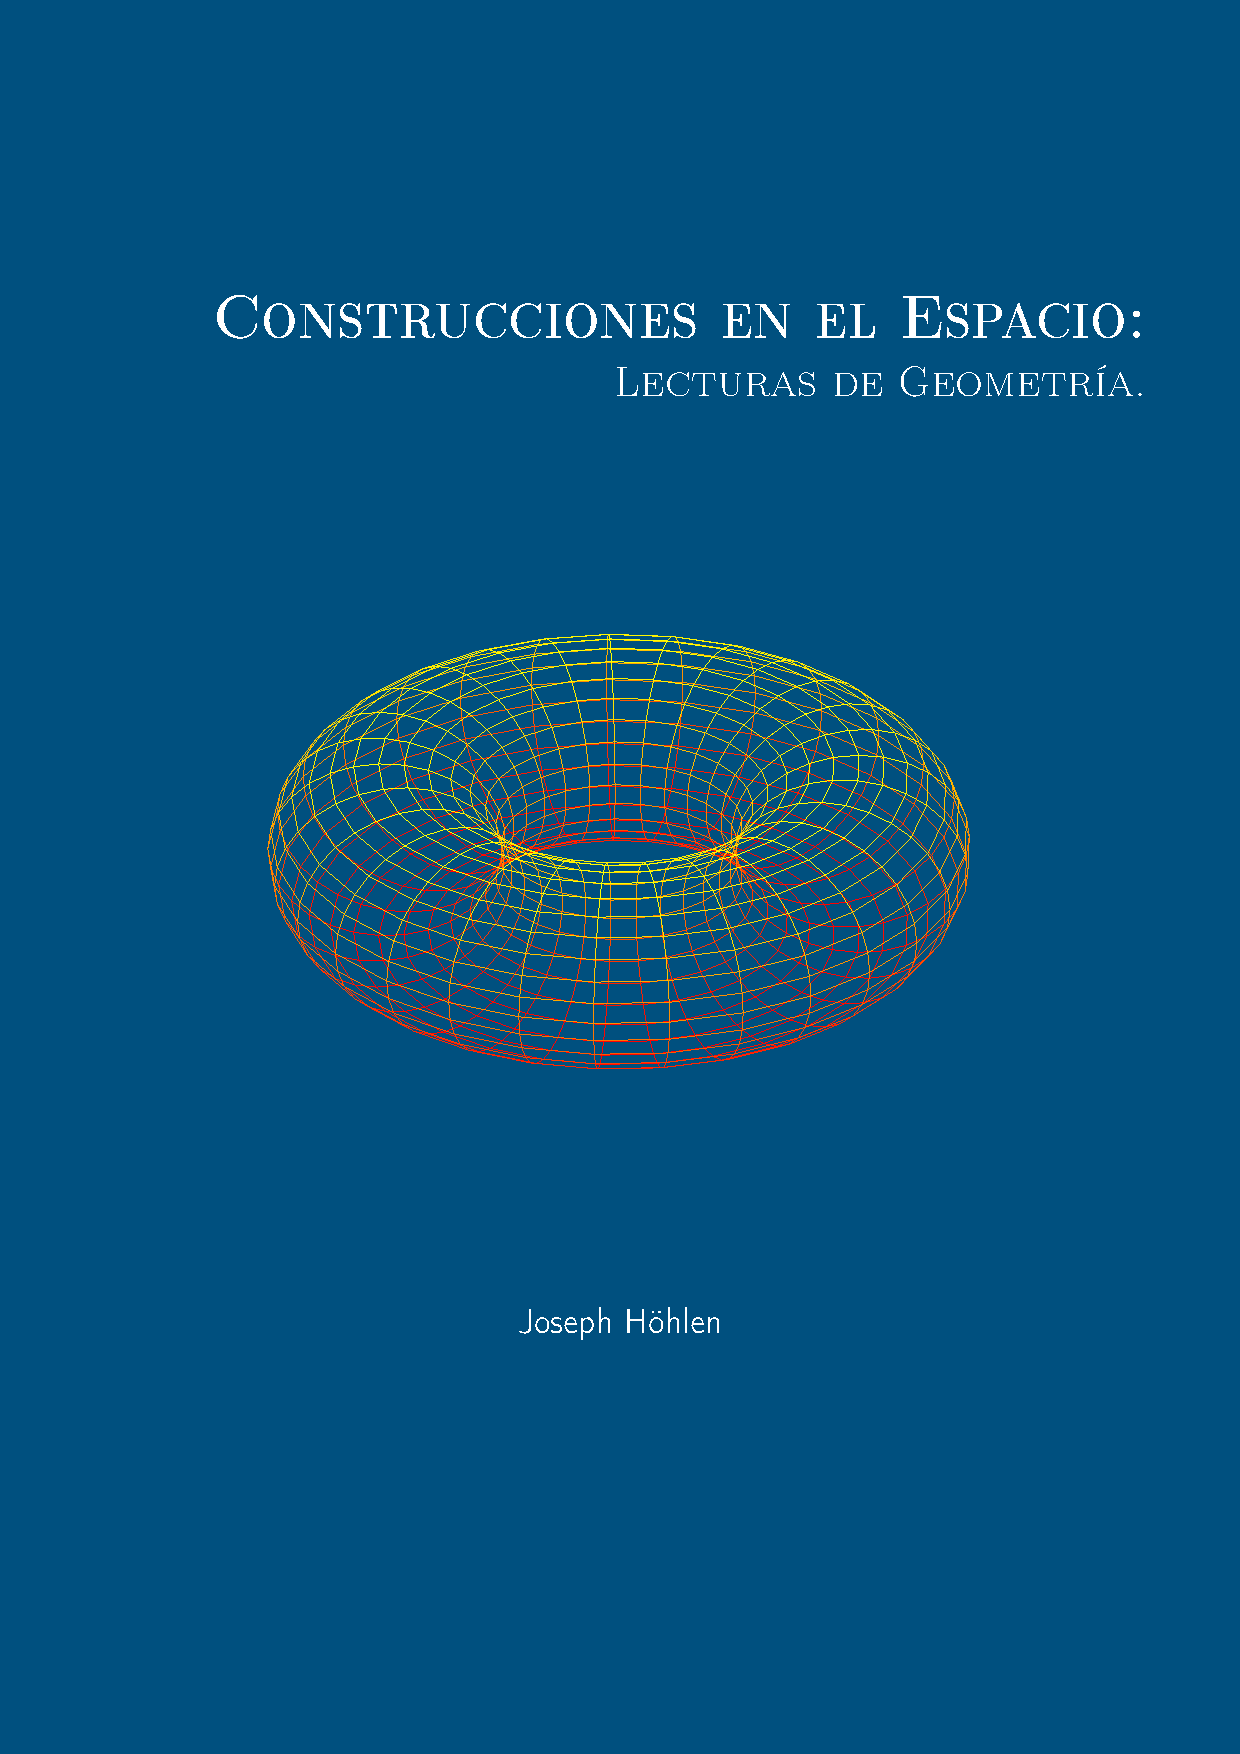
\includepdf[pages=-]{geometria-cover.pdf}

\frontmatter
\maketitle
\tableofcontents
\input{prologo.tex}

\mainmatter
\part{Teoría elemental de números}

\newrefsegment
\input{divisibilidad.tex}
% \input{func-elementales.tex}
\input{congruencias.tex}

\newrefsegment
\subfile{multiplicativas.tex}
% \input{distribucion-primos.tex}

% \part{Teoría Algebraica de Números}

\newrefsegment
\input{enteros-alg.tex}

\newrefsegment
\subfile{valuacion.tex}
\input{ramificacion.tex}

\newrefsegment
\subfile{frac_cont.tex}

\newrefsegment
\input{teoria-kummer.tex}

\part{Geometría diofántica}
\newrefsegment
\input{alturas_proj.tex}

\newrefsegment
\subfile{geometria-num.tex}

\input{roth.tex}
\input{elipticas.tex}

% \part{Teoría de cuerpos de clase}
% \subfile{funciones-L.tex}

\part{Métodos analíticos}
\newrefsegment
\subfile{formas_mod.tex}

\newrefsegment
\input{lineales_log.tex}

\newrefsegment
\input{catalan.tex}

\newrefsegment
\input{abc_et_al.tex}

% \part{Teoría de cuerpos de clase}
\part*{Apéndice}
\appendix

\listofexample
\printnomenclature

% \nocite{*}
% \printbibheading[heading=bibintoc]
% Las fechas empleadas son aquellas de la primera publicación o del primer registro de Copyright.
% \bibbycategory

\printindex

\listoftodos

\end{document}
